% !TEX root = ../report.tex
\section{Das Kamerasystem}
\begin{Spacing}{\mylinespace}

Um eine Navigation in unserer 3D Szene, sowie eine einfache Art der Kalibrierung zu ermöglichen, wurde ein kleines, erweiterbares Kamerasystem entwickelt. Das System besteht aus zwei Hauptkomponenten, der Kamera-Klasse und der Kamerakontroller-Klasse.

\begin{description}
	\item[Kamera] \hfill \\
	Die Kamera-Klasse stellt alle Grundfunktionen einer virtuellen Kamera zur Verfügung. Dazu gehören neben der Translation und der Rotation auch unterschiedliche Arten der Projektion (Perspektivisch, Orthografisch) und verschiedene Kamera-Modi (Orbital, Walk, Fly) zur Navigation. \\\\
	Um den sogenannten \textit{Gimbal Lock} zu vermeiden, welcher bei der Verwendung von \textit{Eulerwinkeln} zur Rotation entstehen kann und in speziellen Fällen den Verlust eines kompletten Freiheitsgrades bewirkt, setzten wir in unserem System auf den Einsatz von \textit{Quantenionen} zur Rotation der Kamera. Diese bieten neben der Vermeidung des \textit{Gimbal Locks} auch eine weitaus effizientere Berechnung der Transformationen.   
	\begin{figure}[h!]
	\centering
	\vspace*{10px}
	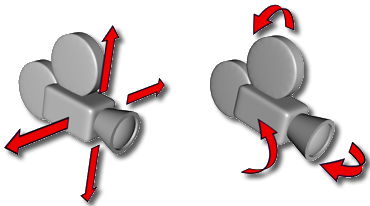
\includegraphics[width=160px]{graphics/cam.png}
	\caption{Grundfunktionen der Kamera.}
	\label{fig:cam}
	\end{figure}
	\item[Kamerakontroller] \hfill \\
	Die Kamerakonroller-Klasse dient als Schnittstelle zwischen der Peripherie und der Kamera und ermöglicht somit eine saubere Trennung zwischen der Verarbeitung von Benutzereingaben und der eigentlichen Funktionalität der Kamera. Abbildung \ref{fig:Camerasystem} zeigt den groben Aufbau des Kamerasystems. 
	\begin{figure}[h!]
	\centering
	\vspace*{30px}
	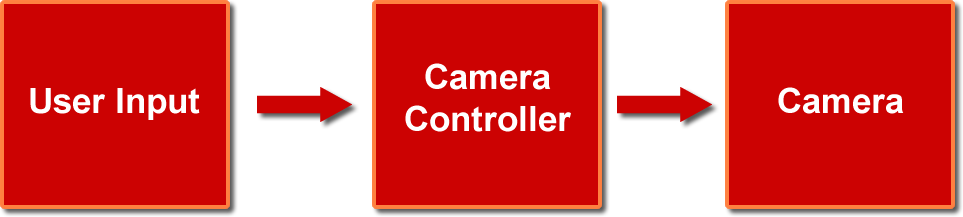
\includegraphics[width=300px]{graphics/camcon.png}
	\caption{Aufbau des Kamerasystems.}
	\label{fig:Camerasystem}
	\end{figure}
\end{description}


\end{Spacing}
\newpage
\clearpage
%% End Of Doc